\section{Graph summarization}

Reducing the complexity of a graph while retaining some of its original properties is known as graph summarization. These summaries often incur an error when running algorithms due to the loss of information. As depicted in \autoref{fig:summarization}, the result of the same algorithm executed on the graph summary will be approximately equal to that of the result of the original graph depending on the compression ratio and a variety of other factors. But usually, when it comes to real-world massive graphs such as social networks, it is enough to obtain approximations instead of the exact answers with a reduced computational cost.

\begin{figure}[H]
    \centering 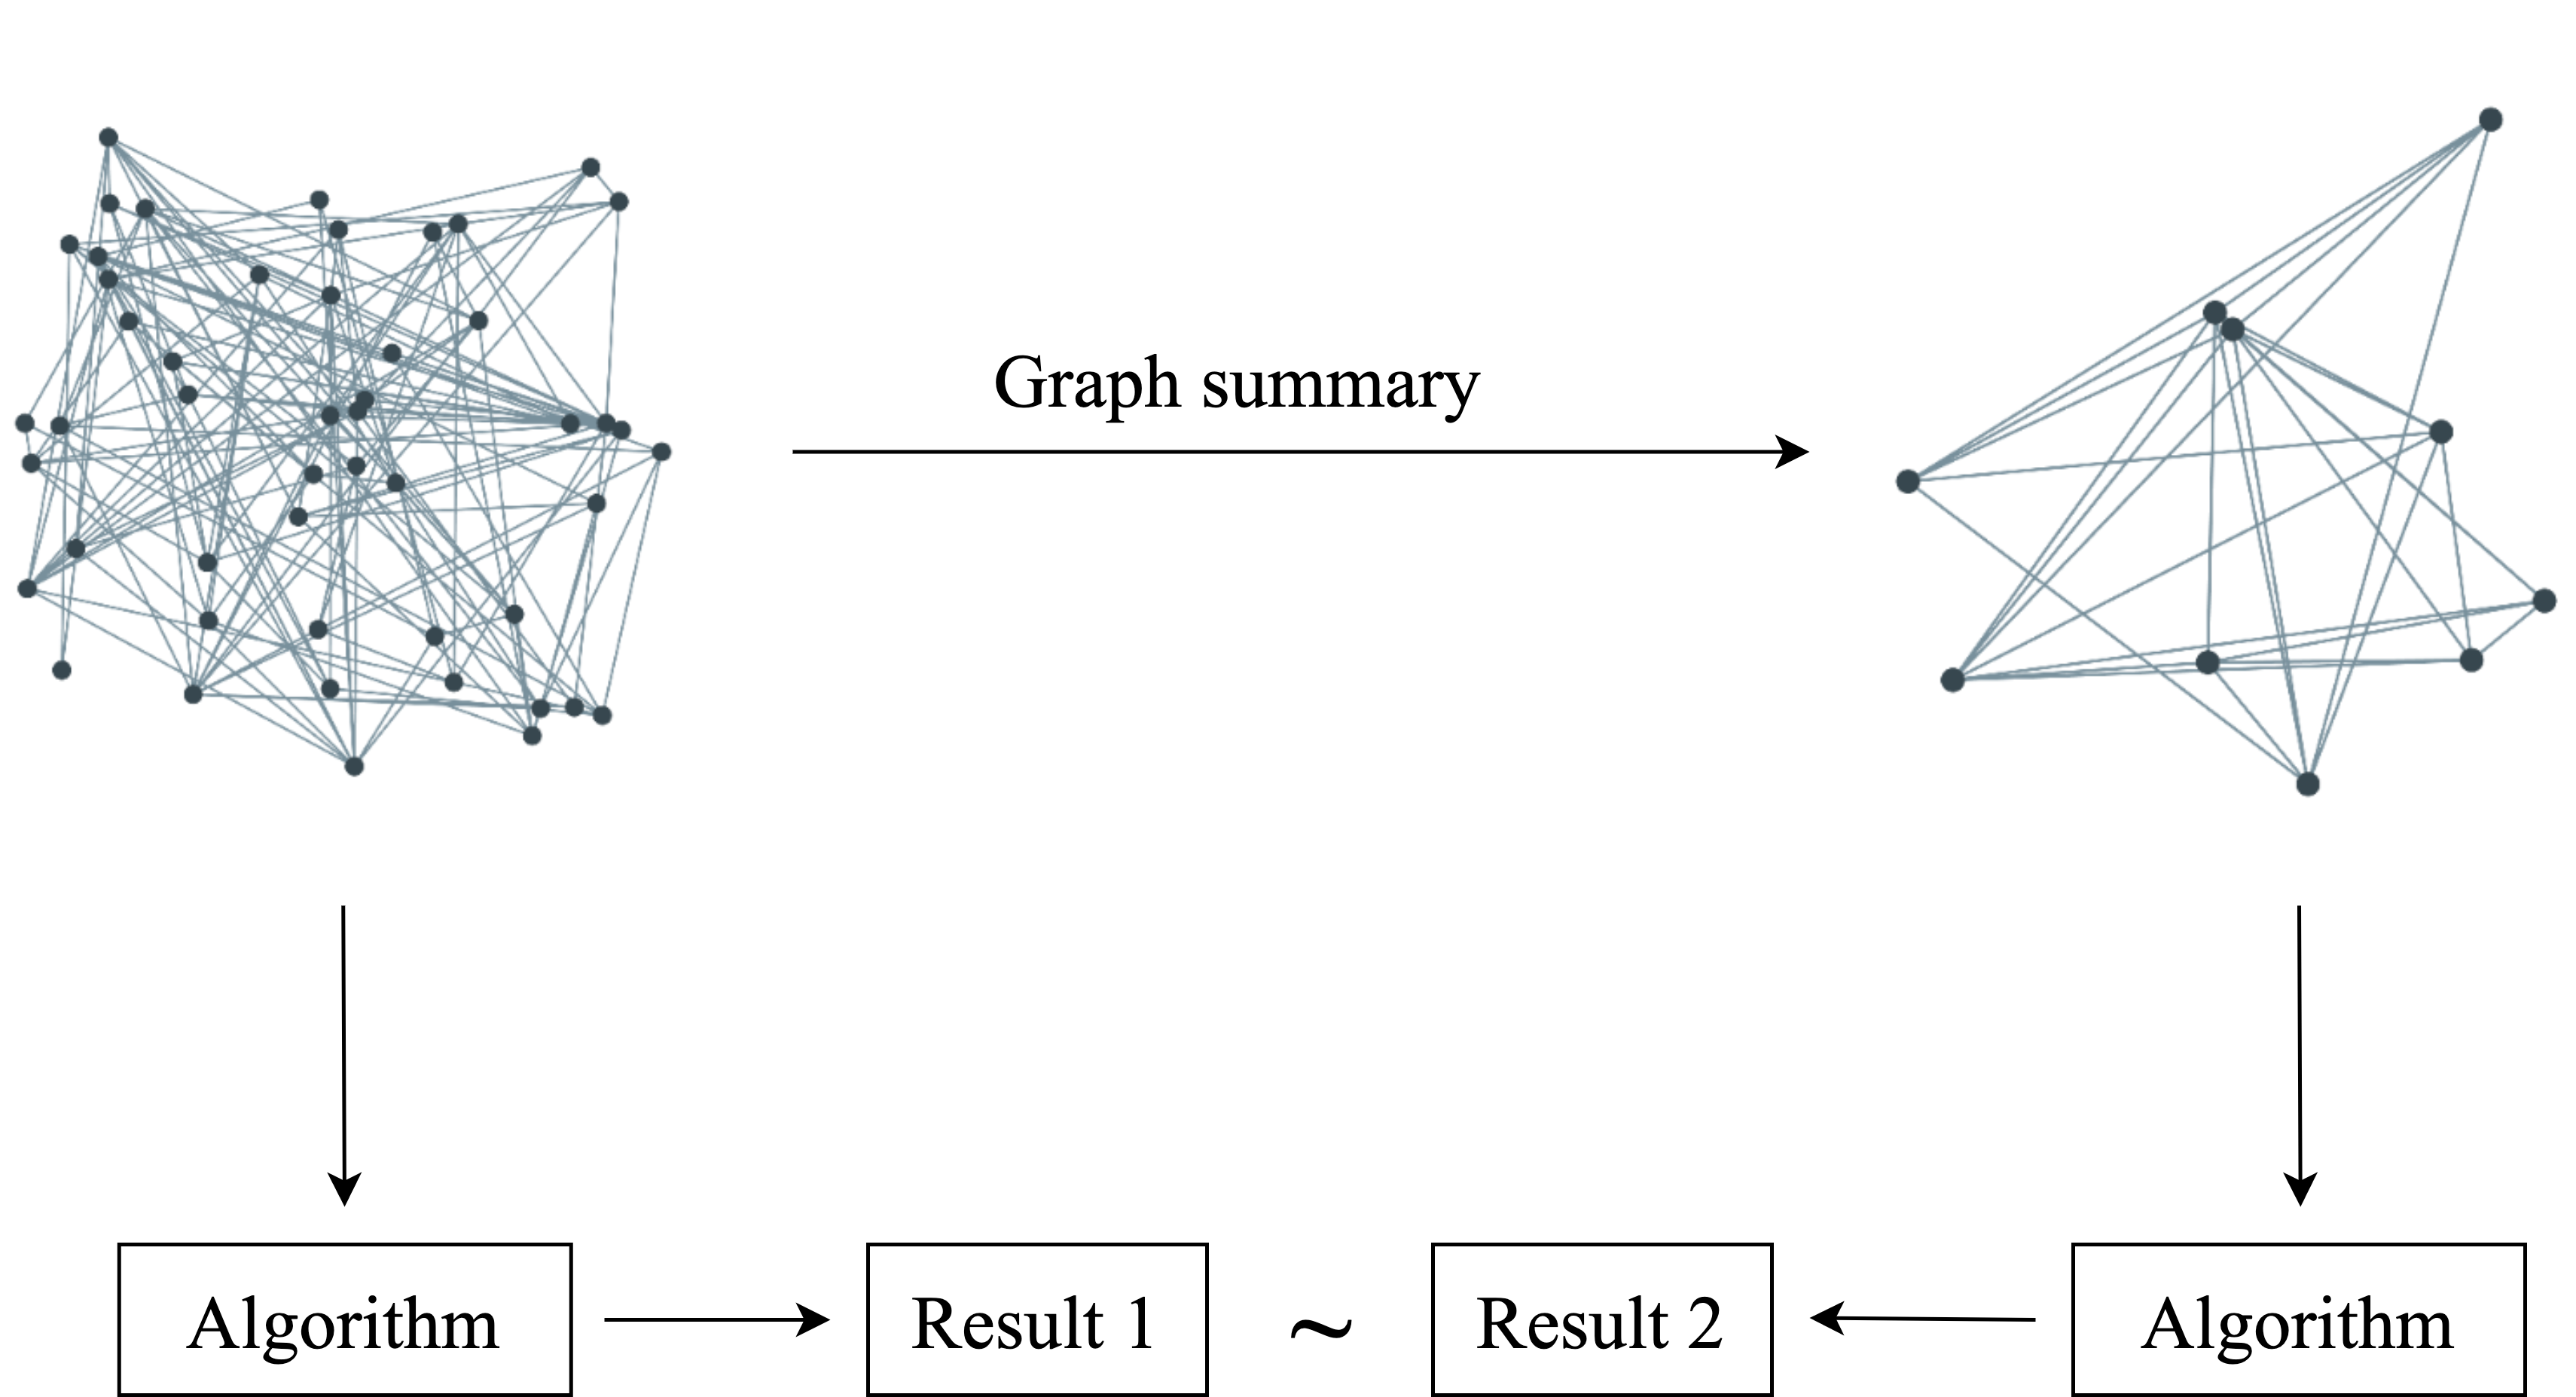
\includegraphics[width=0.7\textwidth]{summarization}
    \caption{Graph summarization}
    \label{fig:summarization}
\end{figure}

\subsection{Benefits of graph summarization}

\paragraph{}
Graph summarization has a wide range of benefits\cite{liu_graph_2018}.

\begin{itemize}
    \item \textbf{Speedup of graph algorithms and queries}\\
          It incurs a huge computational cost to run the regular graph algorithms on massive graphs. Graph summarization always produces a smaller version of the graph, making it easier to run different queries and algorithms on the summarized sketch. The result produced by the summarized sketch will have an accuracy tradeoff when compared with the result that will be given by the original graph\cite{riondato_graph_nodate}. However, the tradeoff is acceptable in some scenarios where the speedup gain is very large.

    \item \textbf{Reduction of data volume and storage}\\
          It takes significant storage to store a large graph on storage media. The space needed for storing the entire graph will be at least \(O(E+V)\). This is not achievable in some scenarios. As an example, an IoT device with limited storage, monitoring a data stream will not be able to store the entire stream in its memory. Graph summarization can be used to reduce the complexity of the original graph in order to reduce the space needed to store the graph\cite{seo_effective_2018}.

    \item \textbf{Visualization\cite{dunne_motif_2013, jin_eco_nodate}}\\
          There are two main issues pertaining to user analysis of large scale streaming graphs. It will be difficult to fit the entire graph in memory so that the visualization algorithm could run on it. Even if the former was achievable, it would be cumbersome to analyse the original graph because of the high number of vertices and edges. Graph summarization could avoid this “hairball” visualization problem\cite{schulz_grooming_2013}.

    \item \textbf{Noise elimination}\\
          Real word graphs are riddled with hidden and erroneous links and labels. Removing the noisy information makes it easier to analyse the graph. Graph summarization could essentially act as a process in filtering out the noise and reveal more interesting features\cite{zhang_discovery-driven_2010}.

    \item \textbf{Privacy preservation}\\
          This can be a crucial step in preserving privacy when releasing the aggregate numbers. Graphs are summarized with the purpose of preserving the privacy of the original dataset\cite{shoaran_zero-knowledge_2013}.
\end{itemize}

\subsection{Applications of graph summarization}

\paragraph{}
Restating the aforementioned, graph summarization has a wide range of benefits and thus used in different industrial and research applications. Apart from these scenarios, there are some other applications of graph summarization such as clustering\cite{cilibrasi_clustering_2005}, classification\cite{hutchison_compression_2006}, community detection\cite{chakrabarti_fully_nodate}, outlier detection\cite{smets_odd_2011, akoglu_opavion_2012}, pattern set mining\cite{mampaey_tell_2011} and finding sources of infection in large graphs\cite{prakash_spotting_2012}.

\paragraph{}
During this research, our aim lies in query optimization through graph summarization.

\subsection{Challenges of graph summarization}

\paragraph{}
There are many challenges involving in graph summarization\cite{liu_graph_2018}.

\begin{itemize}
    \item \textbf{Data volume}\\
          Graph summarization primarily intends to deal with the large volume of data. Therefore handling the original dataset in order to create the summary sketch itself is a cumbersome task.

    \item \textbf{Complexity of data}\\
          Some graphs can be heterogeneous in nature, making it increasingly more difficult to summarize the graph. Considering the heterogeneity of the nodes during the summarization may lead to a complex architecture\cite{kivela_multilayer_2014}.

    \item \textbf{Definition of interestingness}\\
          Definition of interestingness depends on the application scenario and user preference. It is difficult to determine the acceptable tradeoffs for a specific summarization without the domain knowledge.

    \item \textbf{Evaluation}\\
          There are a number of parameters that can be used for the evaluation of graph summaries. A summary is considered good if it efficiently supports both the local and global queries with high accuracy. But in a scenario where visualization is involved, qualitative criteria would have to be used for evaluation as it is subjective to the opinion of the domain experts.

    \item \textbf{Change over time}\\
          Usually, real-world graphs are streaming, thus the summaries should also evolve with time\cite{leskovec_graphs_2005}.
\end{itemize}

\subsection{Types of graph summarization}
\label{section:sumtypes}

\paragraph{}
Graph summarization methods can be categorized according to various criteria.

\paragraph{}
One classification is, according to the nature of the input data; static graph summarization and streaming graph summarization. Static graphs do not evolve with time, thus making it impossible to use the same methods to summarize both static and streaming graphs. Due to their dynamic nature, an extra effort has to be spent on summarizing the streaming graphs. In this research, we will only focus on summarizing streaming graphs.

\paragraph{}
Summaries can also be classified considering the nature of the input graph; homogeneous and heterogeneous. We will only consider about homogenous summaries during this research.

\paragraph{}
There are a few core techniques used when summarizing graphs\cite{liu_graph_2018}.

\begin{itemize}
    \item \textbf{Grouping or aggregation based}\\
          Nodes are aggregated into ‘supernodes’ in order to reduce the complexity of the original graph. Edge-grouping methods aggregate multiple edges into single edges.

    \item \textbf{Bit compression based}\\
          Bit compression minimizes the number of bits needed to store the input graph. There are lossy compression methods as well as lossless compression methods.

    \item \textbf{Simplification or sparsification based}\\
          This approach removes the less important nodes and edges producing a sparsified graph.

    \item \textbf{Influence based}\\
          Influence based summarization aims to provide insights into the influence propagation of a graph. This type of summarization can be specially useful in scenarios where social networks are considered.
\end{itemize}

\subsection{Streaming graph summarization}

\paragraph{}
Summarizing graph streams is more difficult than summarizing a static graph due to the constant flow of data. Underlying original graph is constantly updated while it is being summarized. Therefore the summarization process has to be done in realtime. Almost any static graph summarization technique could be used with streaming graph snapshots within specific time frames. However, mining information using aggregate time snapshots of data could very well be an unrealistic goal in a massive streaming graph. Thus sophisticated sparsification techniques have to be derived in order to summarize streaming graphs.

\subsubsection{CountMin\cite{cormode_improved_2003}}

\paragraph{}
CountMin could be considered as the pioneering work in summarizing data streams which are directly related to our research. CountMin is a data structure that is used for frequency approximation queries. The underlying idea behind the CountMin data structure is to hash the aggregated frequencies of the edges using multiple hash functions into predefined blocks as indicated in \autoref{fig:countmin}. A fixed-size will be stated at the time of the creation of the CountMin sketch and irrespective of the volume of data stored, the size of the sketch does not have to be changed. The major drawback in following this procedure is that the error of the queries reduce as more and more data is introduced to the sketch. However, despite these weaknesses, CountMin can be considered as a good generalized sketch at the time as many other sketches described in the literature are good for one single pre-specified aggregate computation. Therefore CountMin approach is not restricted to streaming graphs but other applications as well\cite{cormode_improved_2003}.

\begin{figure}[H]
    \centering 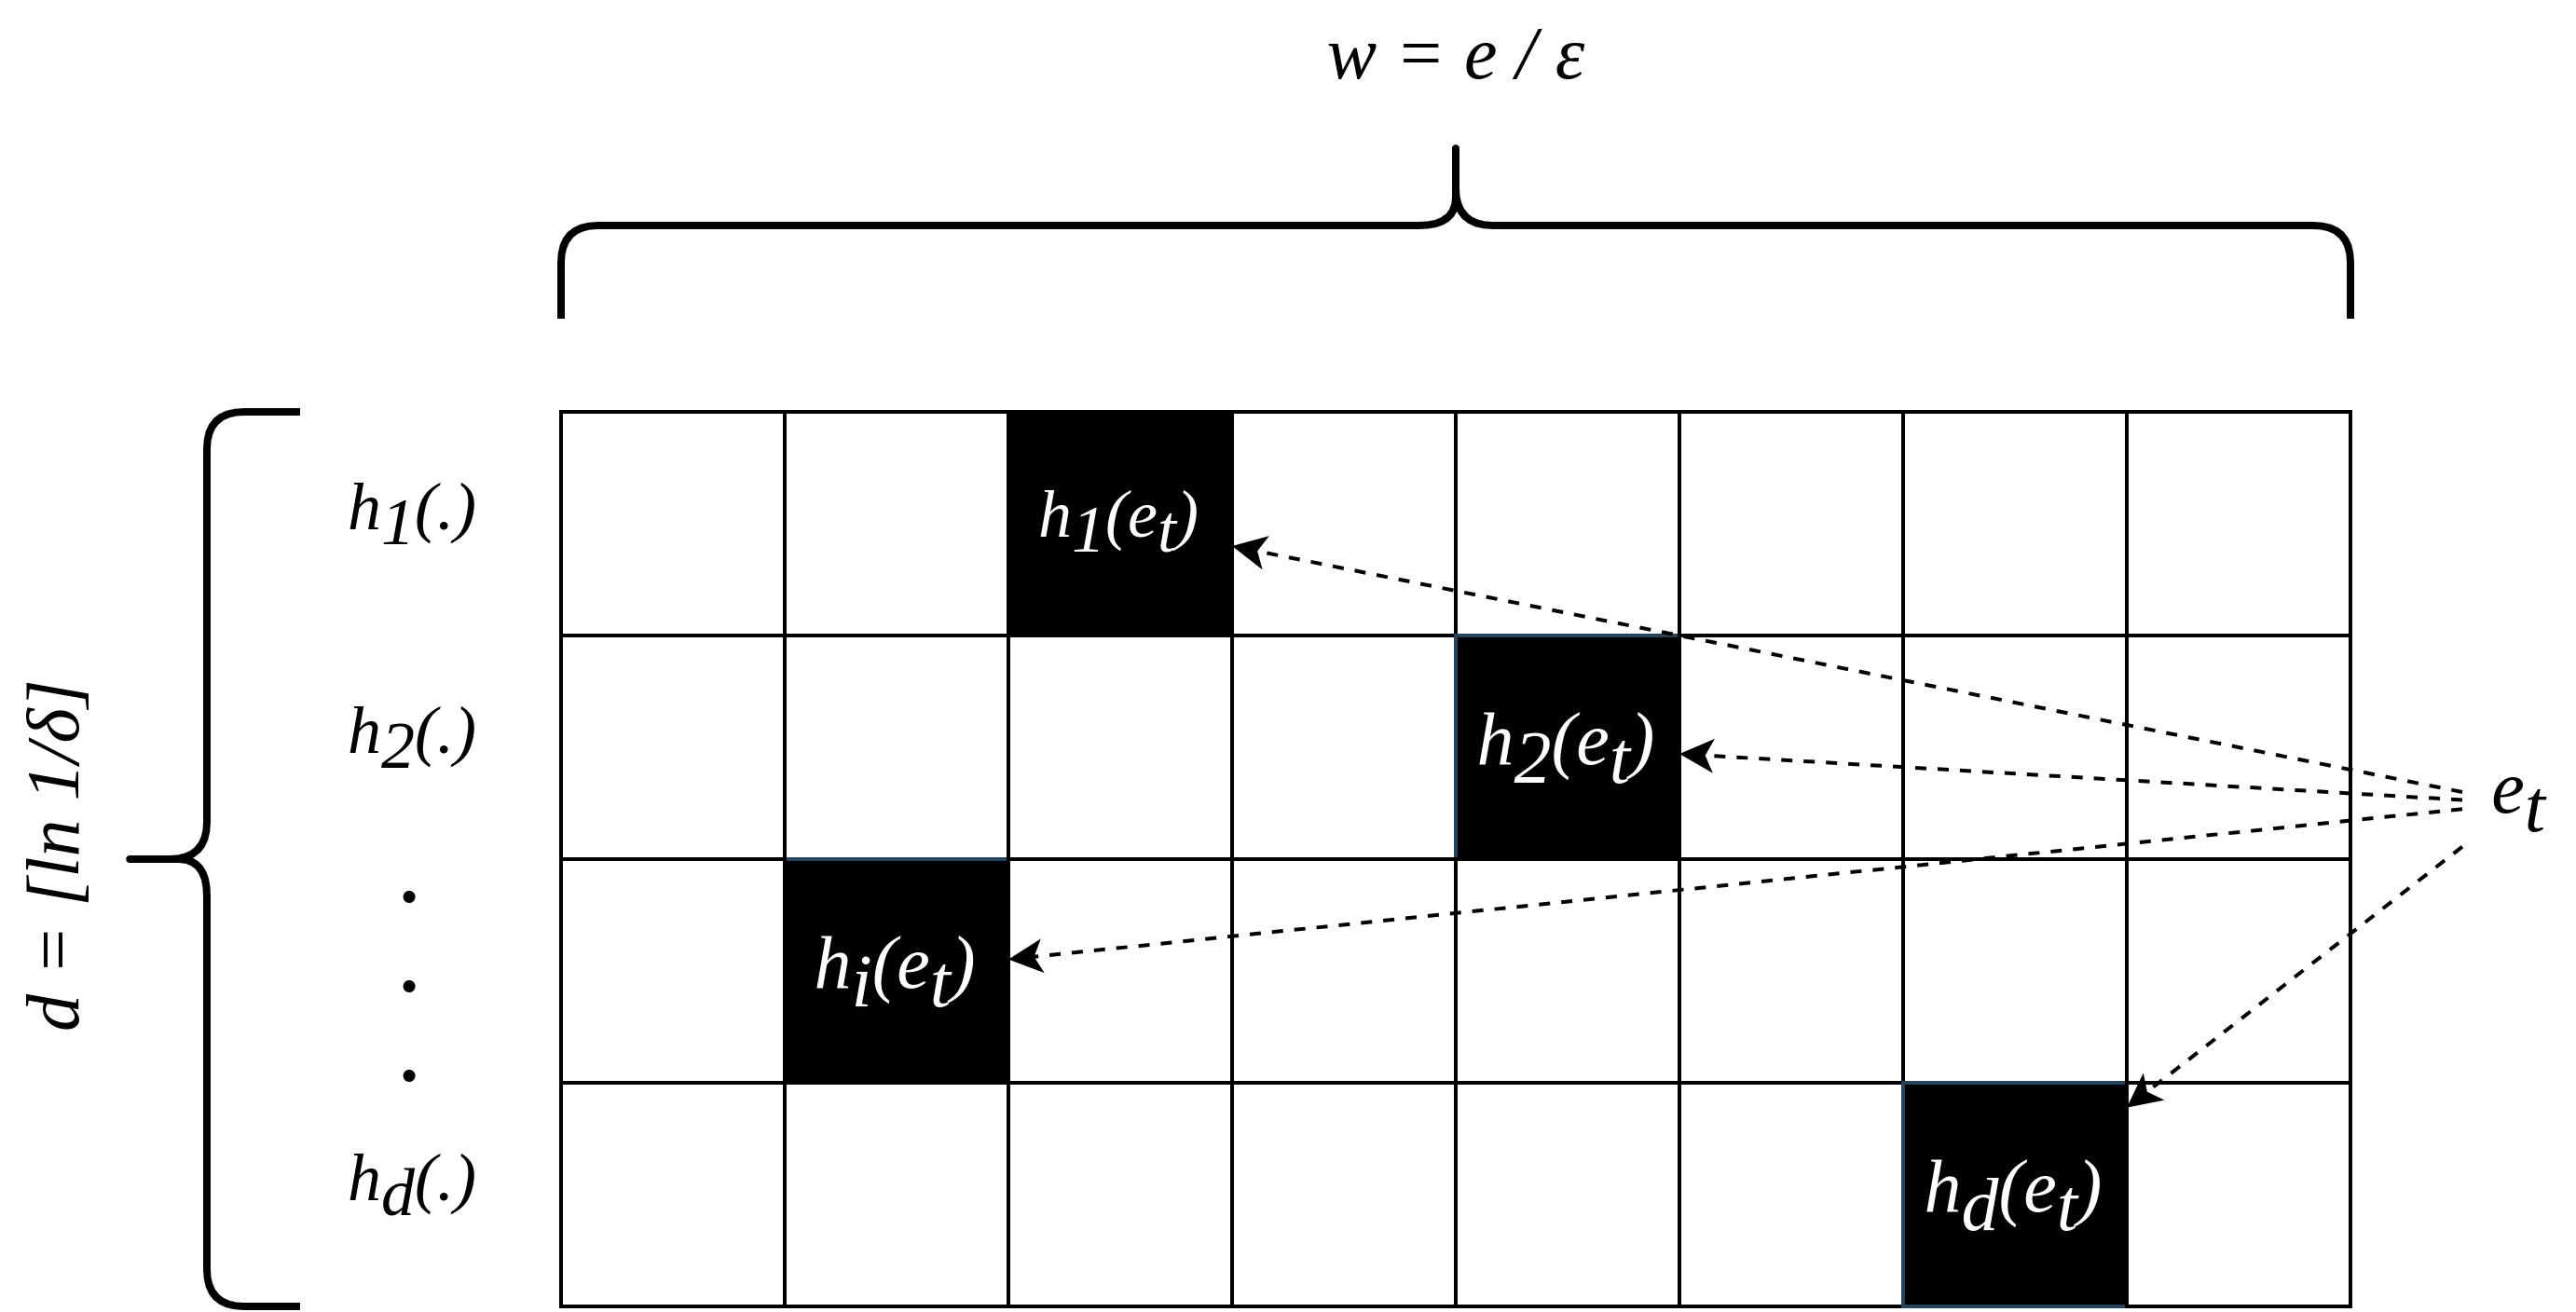
\includegraphics[width=\textwidth]{countmin}
    \caption{CountMin sketch}
    \label{fig:countmin}
\end{figure}

\subsubsection{gSketch\cite{zhao_gsketch:_2011}}

\paragraph{}
gSketch is an extension of CountMin data structure. But unlike CountMin sketch, this is specifically geared towards summarizing graph streams. gSketch is based on one of the two assumptions that,

\begin{itemize}
    \item A graph stream sample is available.
    \item Both graph stream sample and a query workload sample are available.
\end{itemize}

\paragraph{}
As per the previous sketching technique, CountMin, a global sketch is created for the entire graph stream. The disadvantage of this method is that any structural properties present in the graph stream are completely ignored throughout this process. gSketch tries to avoid by considering the underlying structural properties of the graph.

\paragraph{}
The speciality of gSketch is to pre-process the stream samples and creating sketch partitions as indicated in \autoref{fig:gsketch}. Its goal is to maintain sufficient frequency uniformity within each localized sketch so that the query estimation can be optimized over the entire graph stream.

\begin{figure}[H]
    \centering 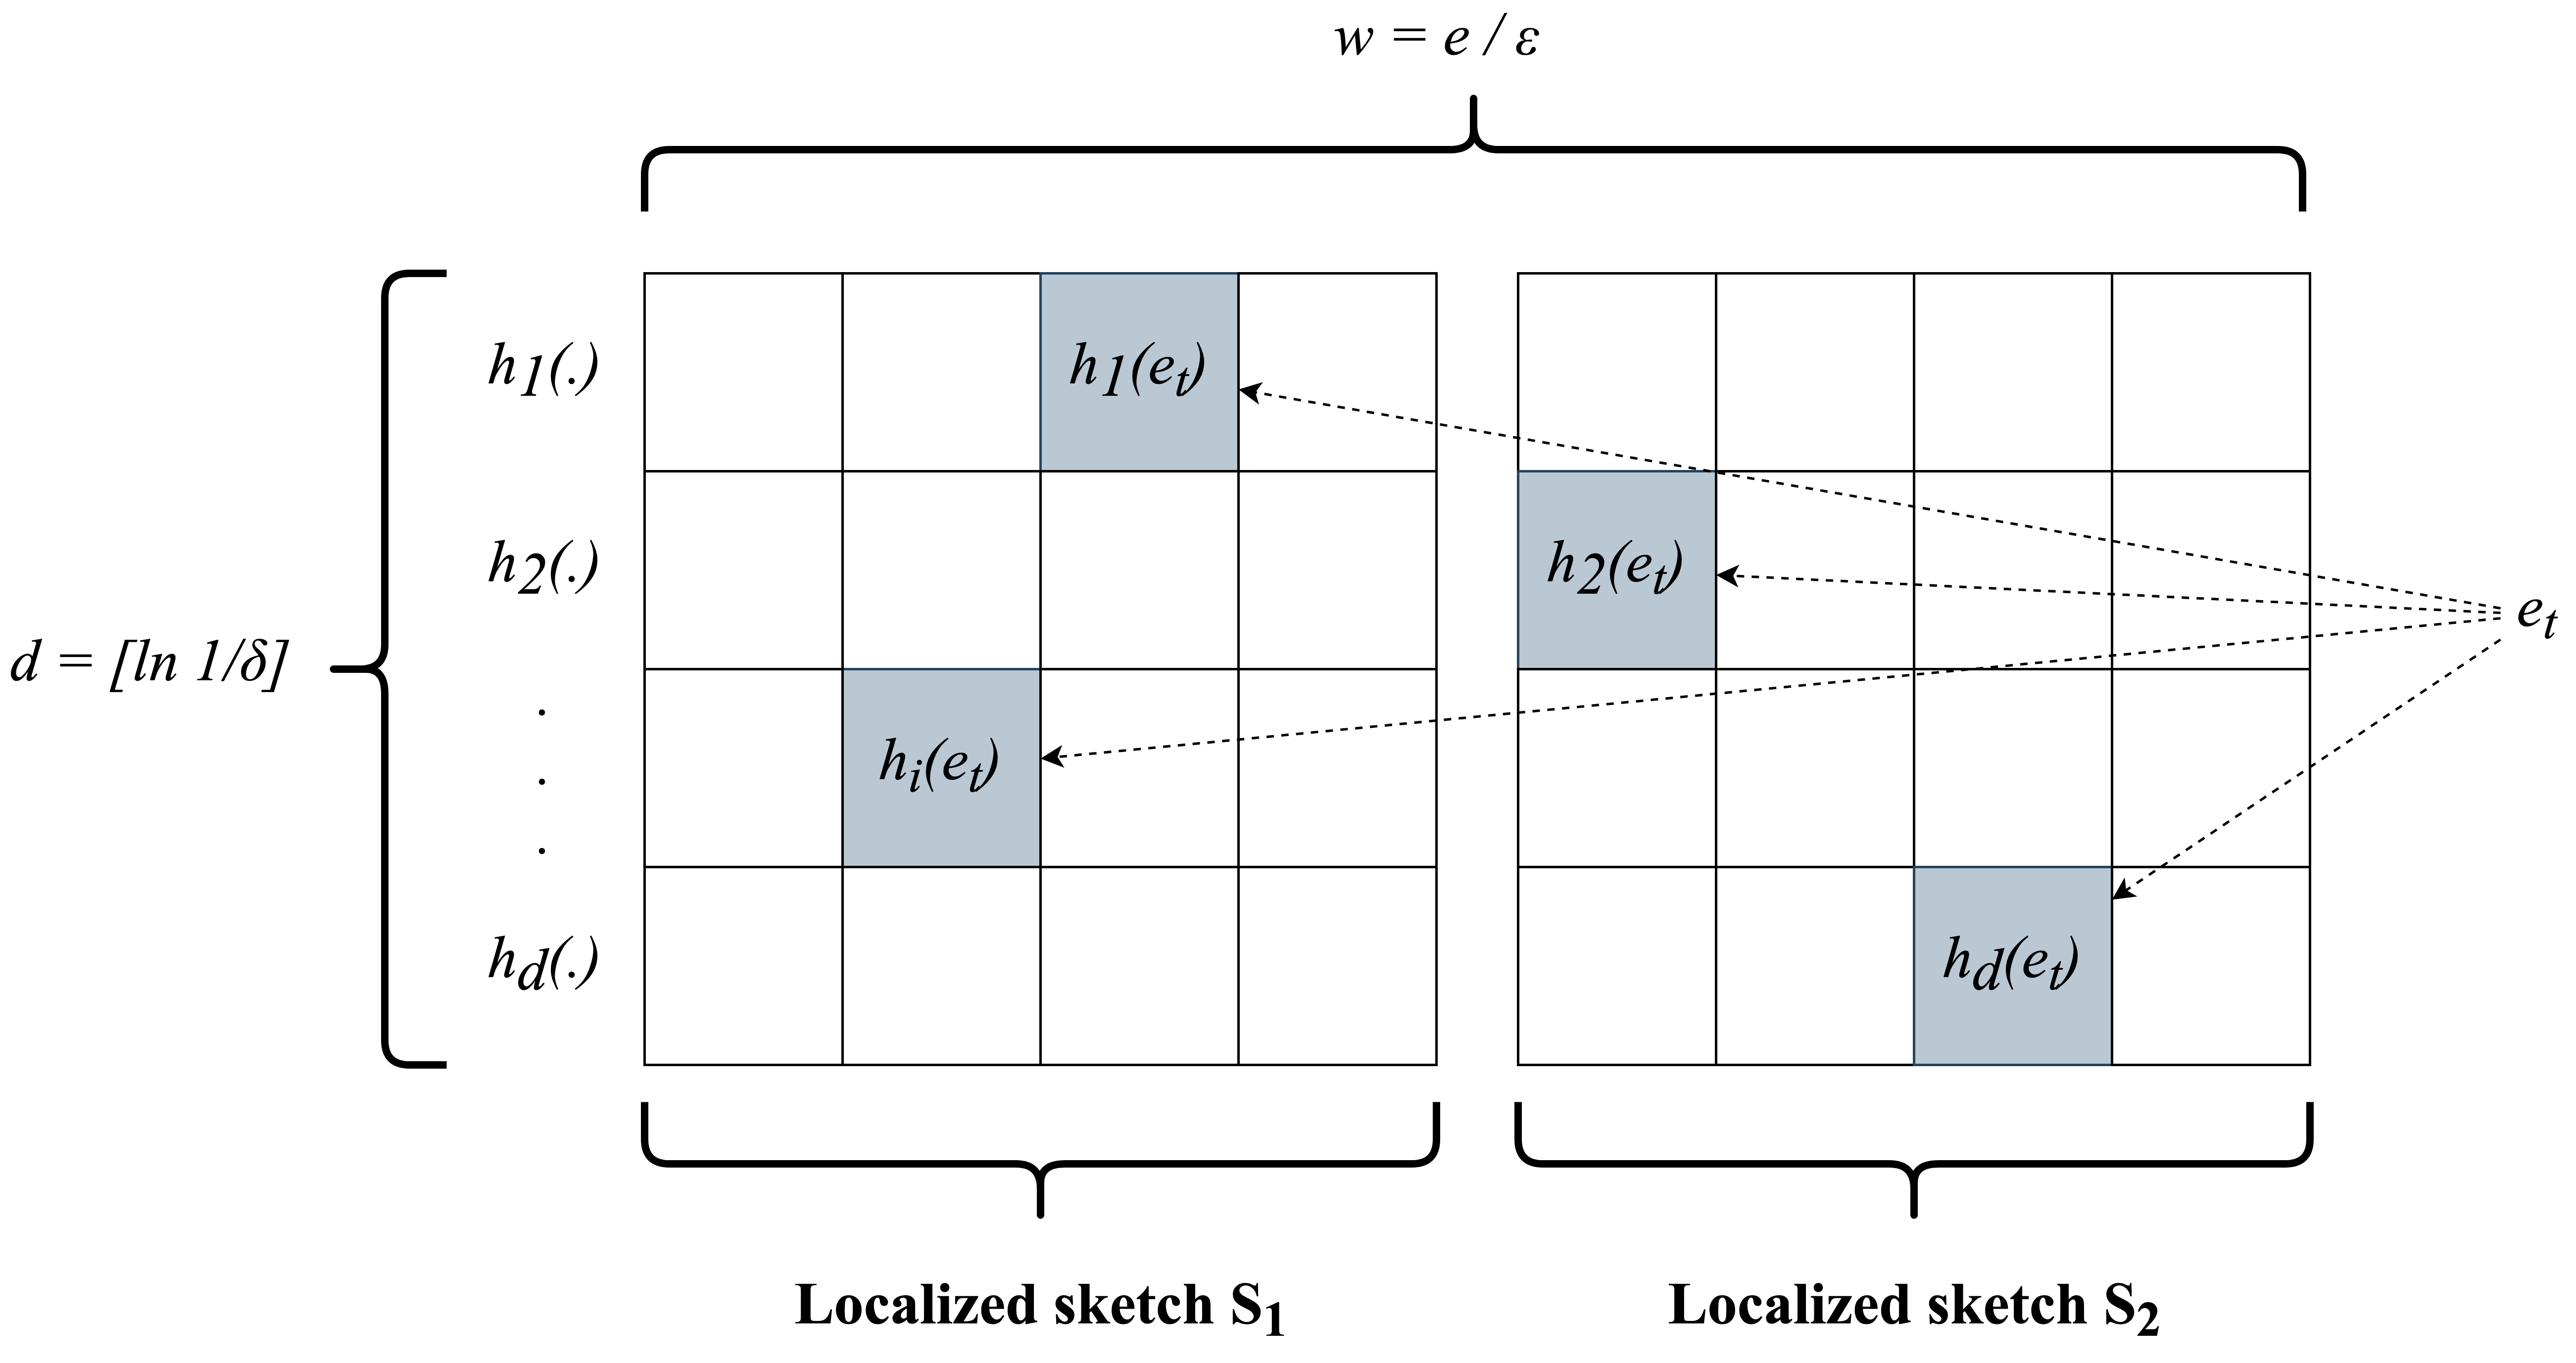
\includegraphics[width=\textwidth]{gsketch}
    \caption{gSketch sketch}
    \label{fig:gsketch}
\end{figure}

\subsubsection{TCM\cite{tang_graph_2016}}

\paragraph{}
Approximate Frequency Count sketches store aggregated frequencies of edges in summarized form. When there is a graph stream as indicated in \autoref{fig:afc_sample_stream}, its summarized node sketch and edge sketch would be the mappings described by \autoref{fig:afc_node_sketch} and \autoref{fig:afc_edge_sketch} respectively.

\begin{figure}[H]
    \centering 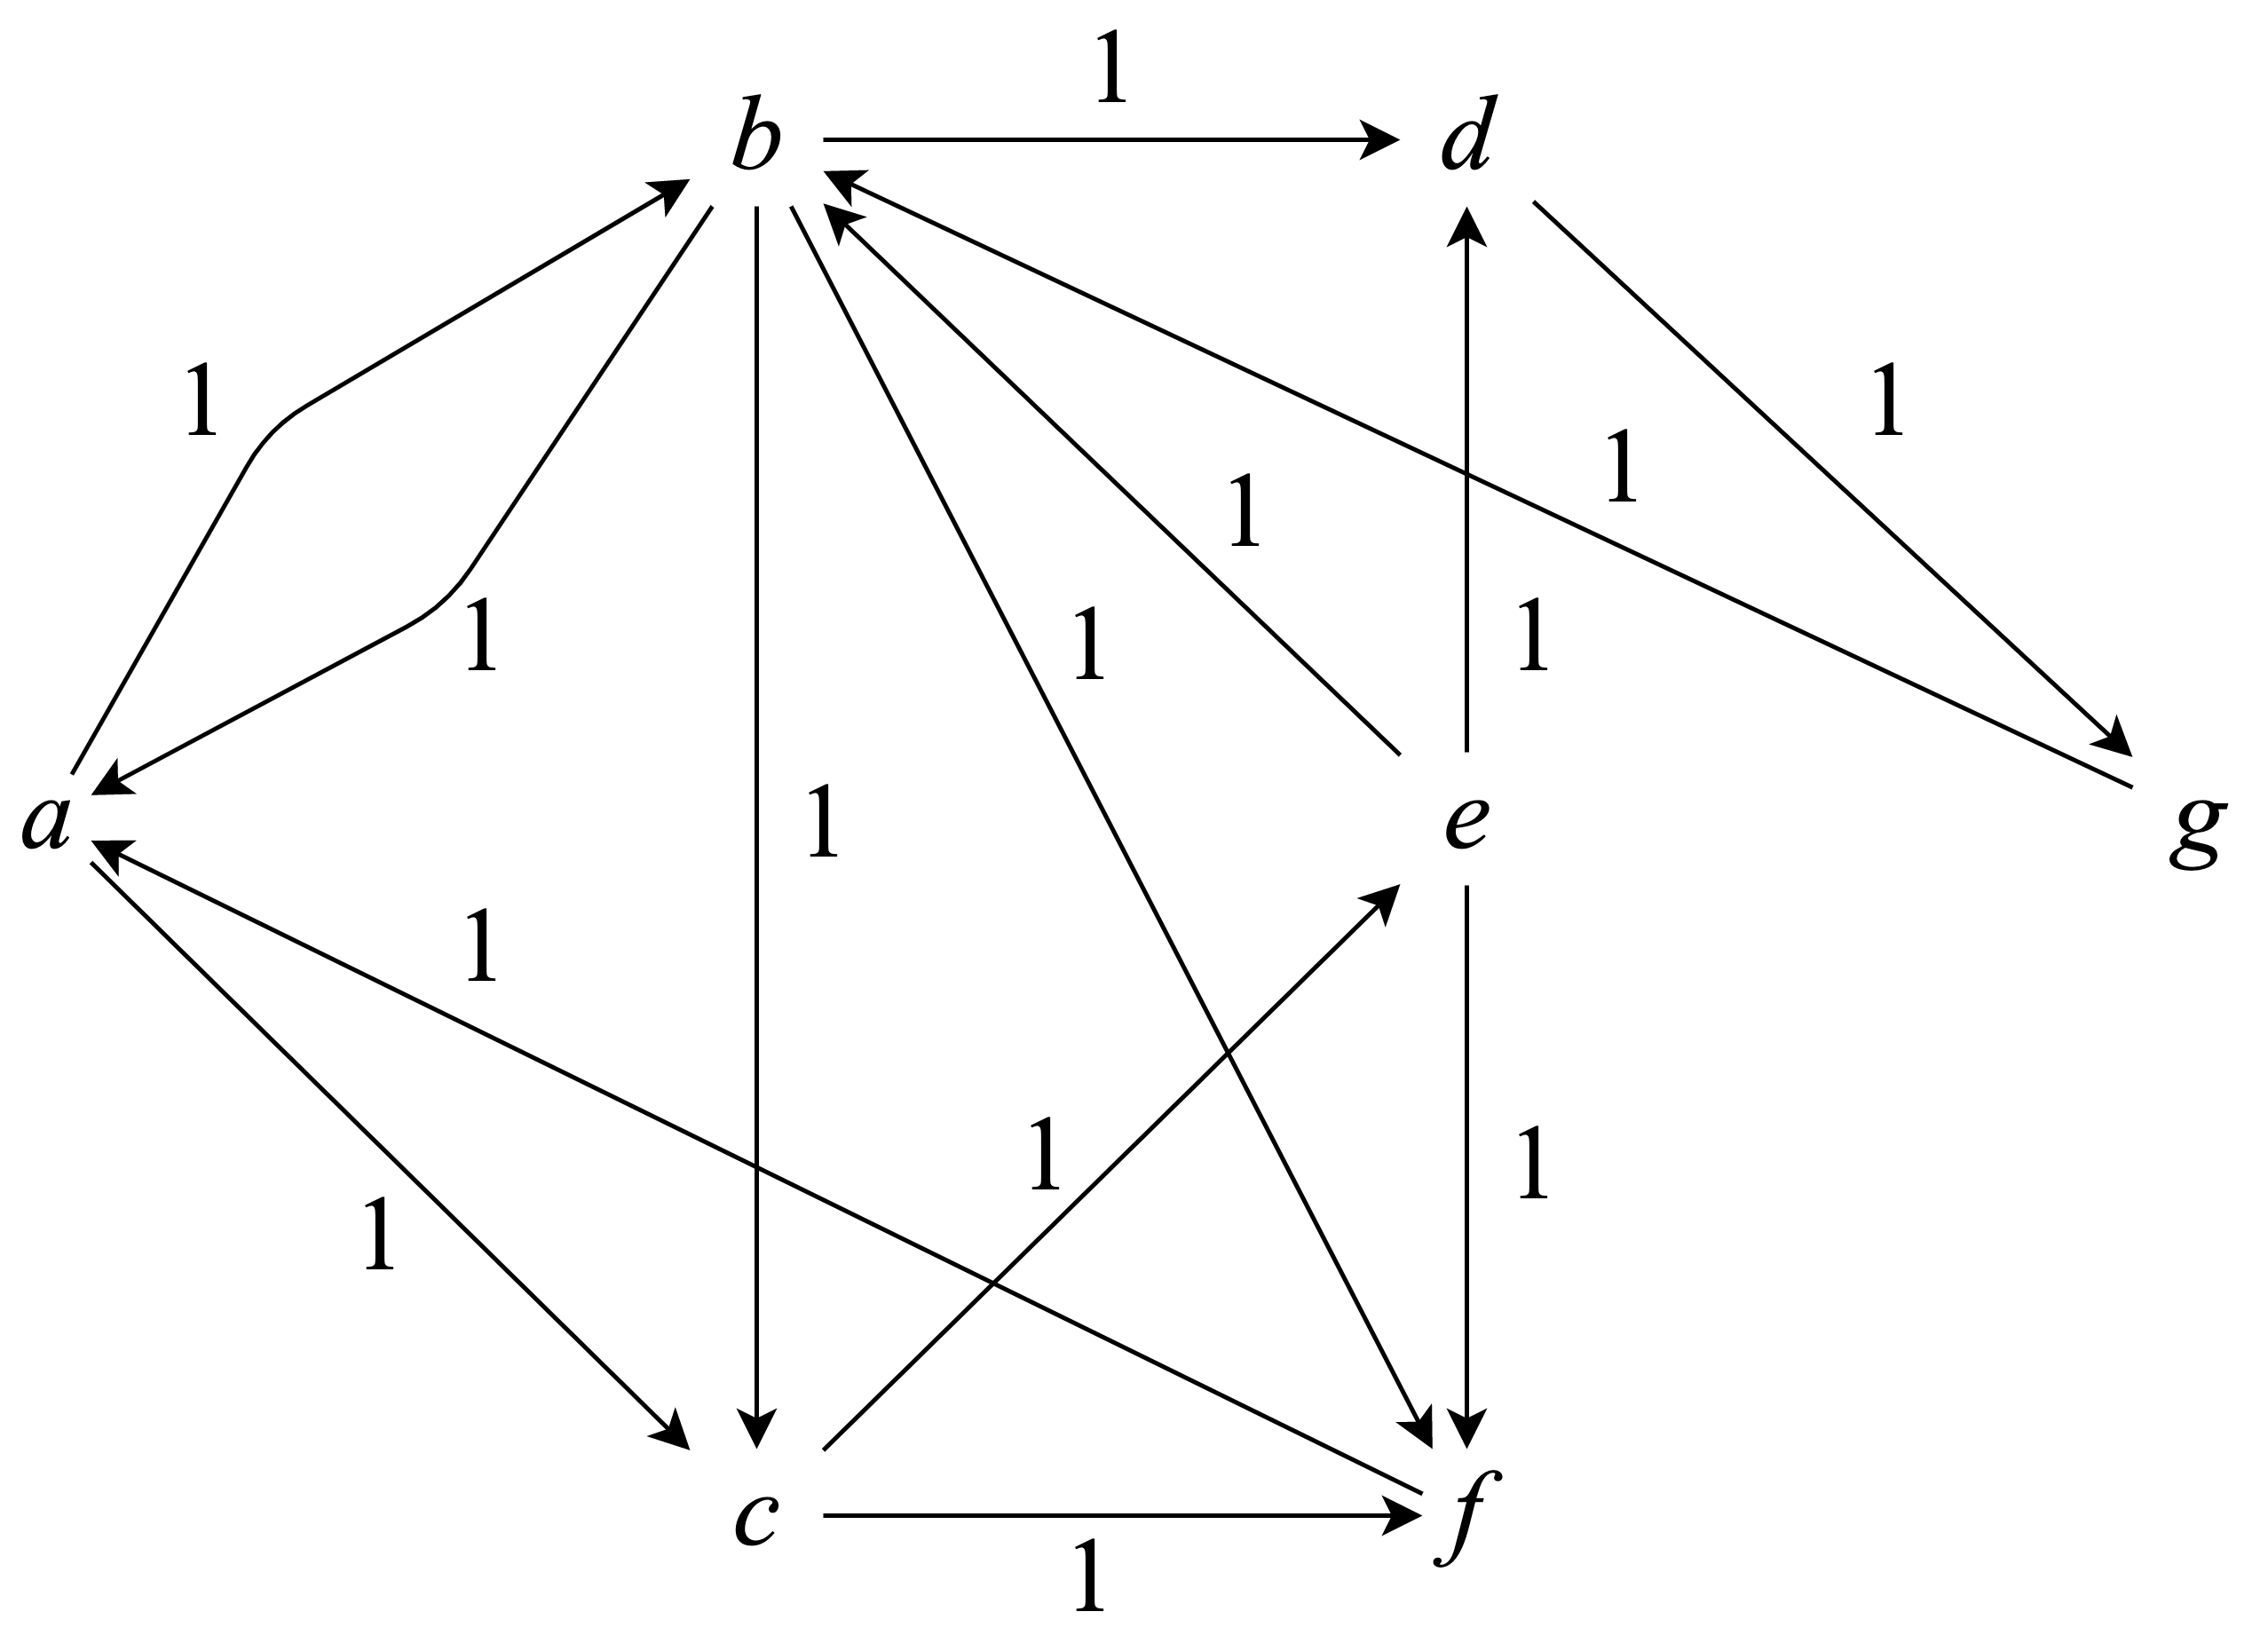
\includegraphics[width=0.5\textwidth]{afc_sample_stream}
    \caption{A sample graph stream}
    \label{fig:afc_sample_stream}
\end{figure}

\begin{figure}[H]
    \centering 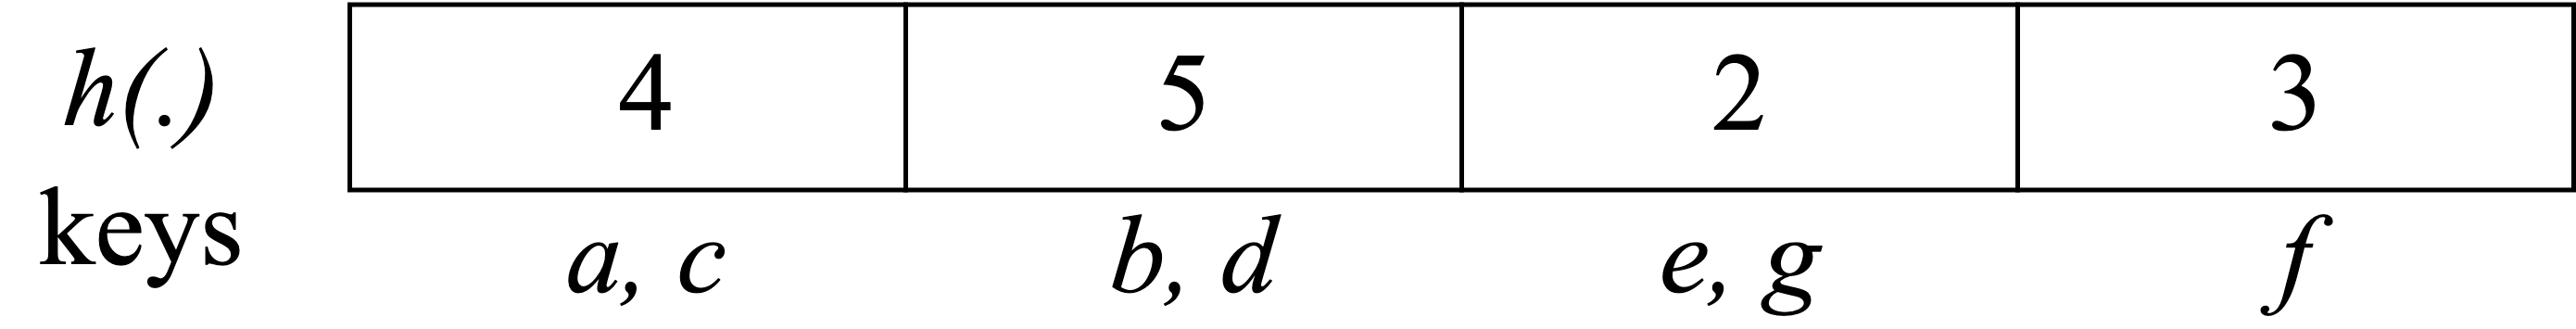
\includegraphics[width=0.5\textwidth]{afc_node_sketch}
    \caption{Node sketch}
    \label{fig:afc_node_sketch}
\end{figure}

\begin{figure}[H]
    \centering 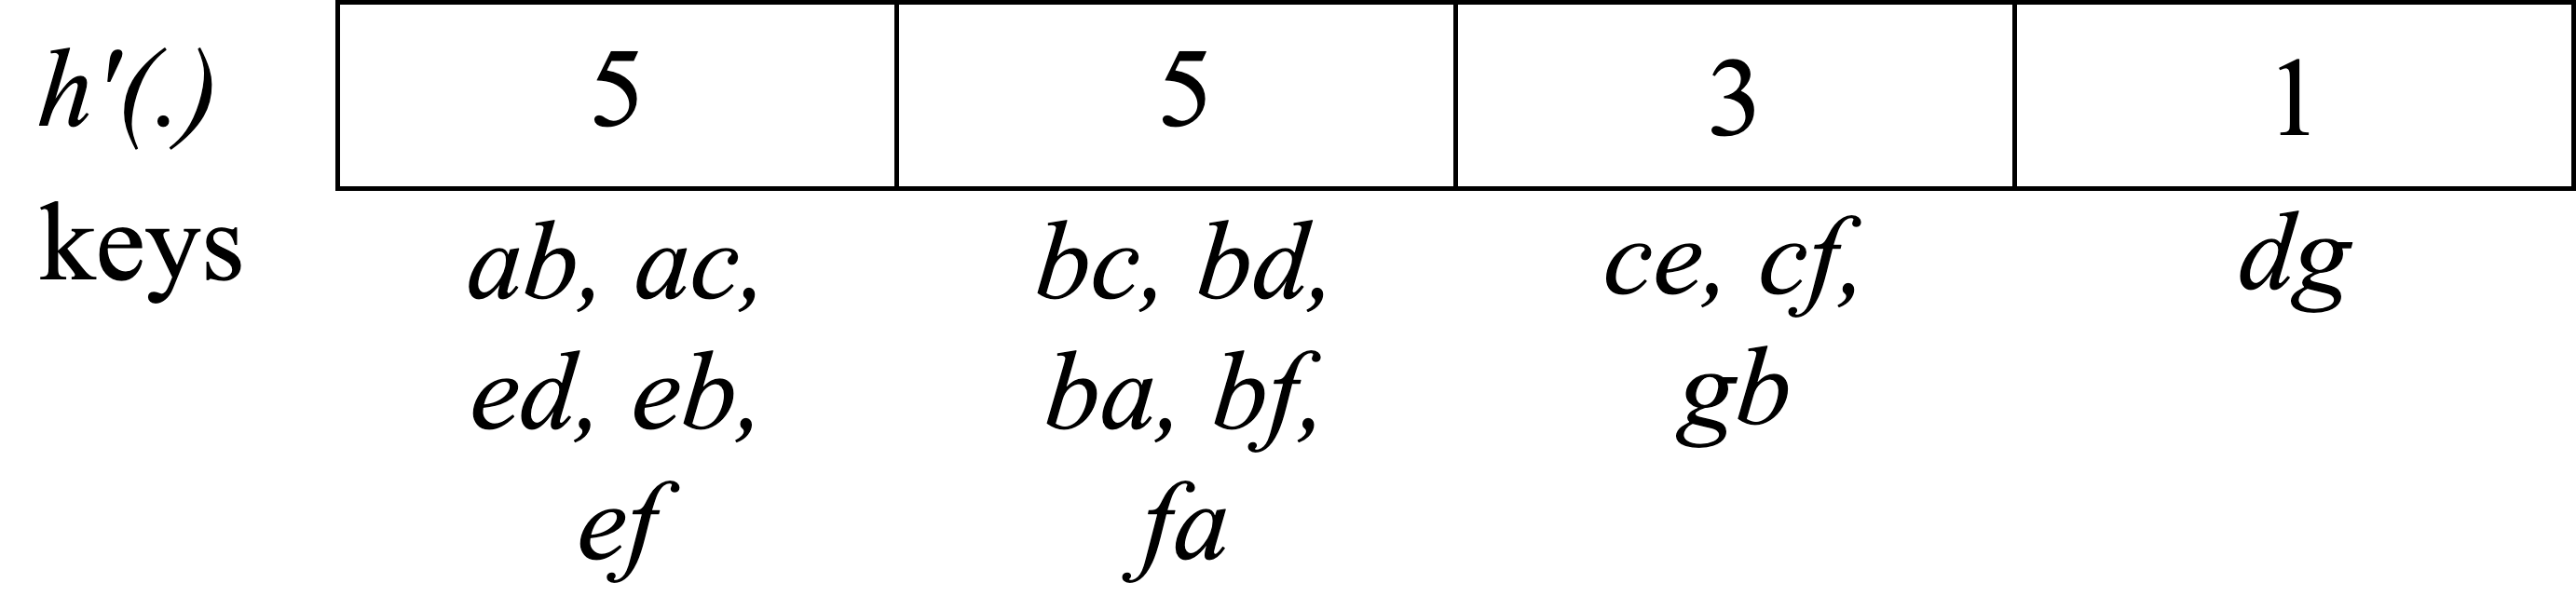
\includegraphics[width=0.5\textwidth]{afc_edge_sketch}
    \caption{Edge sketch}
    \label{fig:afc_edge_sketch}
\end{figure}

\paragraph{}
A disadvantage posed by all the approximate frequency count sketches like CountMin or gSketch is that they do not store the locality of the nodes. Therefore they cannot be used for conditional node queries or queries involving node connectivity. If these queries were to be run, at least some of the information about the locality of nodes has to be retained in the graph synopses. TCM can summarize both node and edge information in constant time. Because of that, it can answer a wide range of queries, unlike its predecessors. The structure of a TCM sketch is depicted in \autoref{fig:tcm}.

\begin{figure}[H]
    \centering 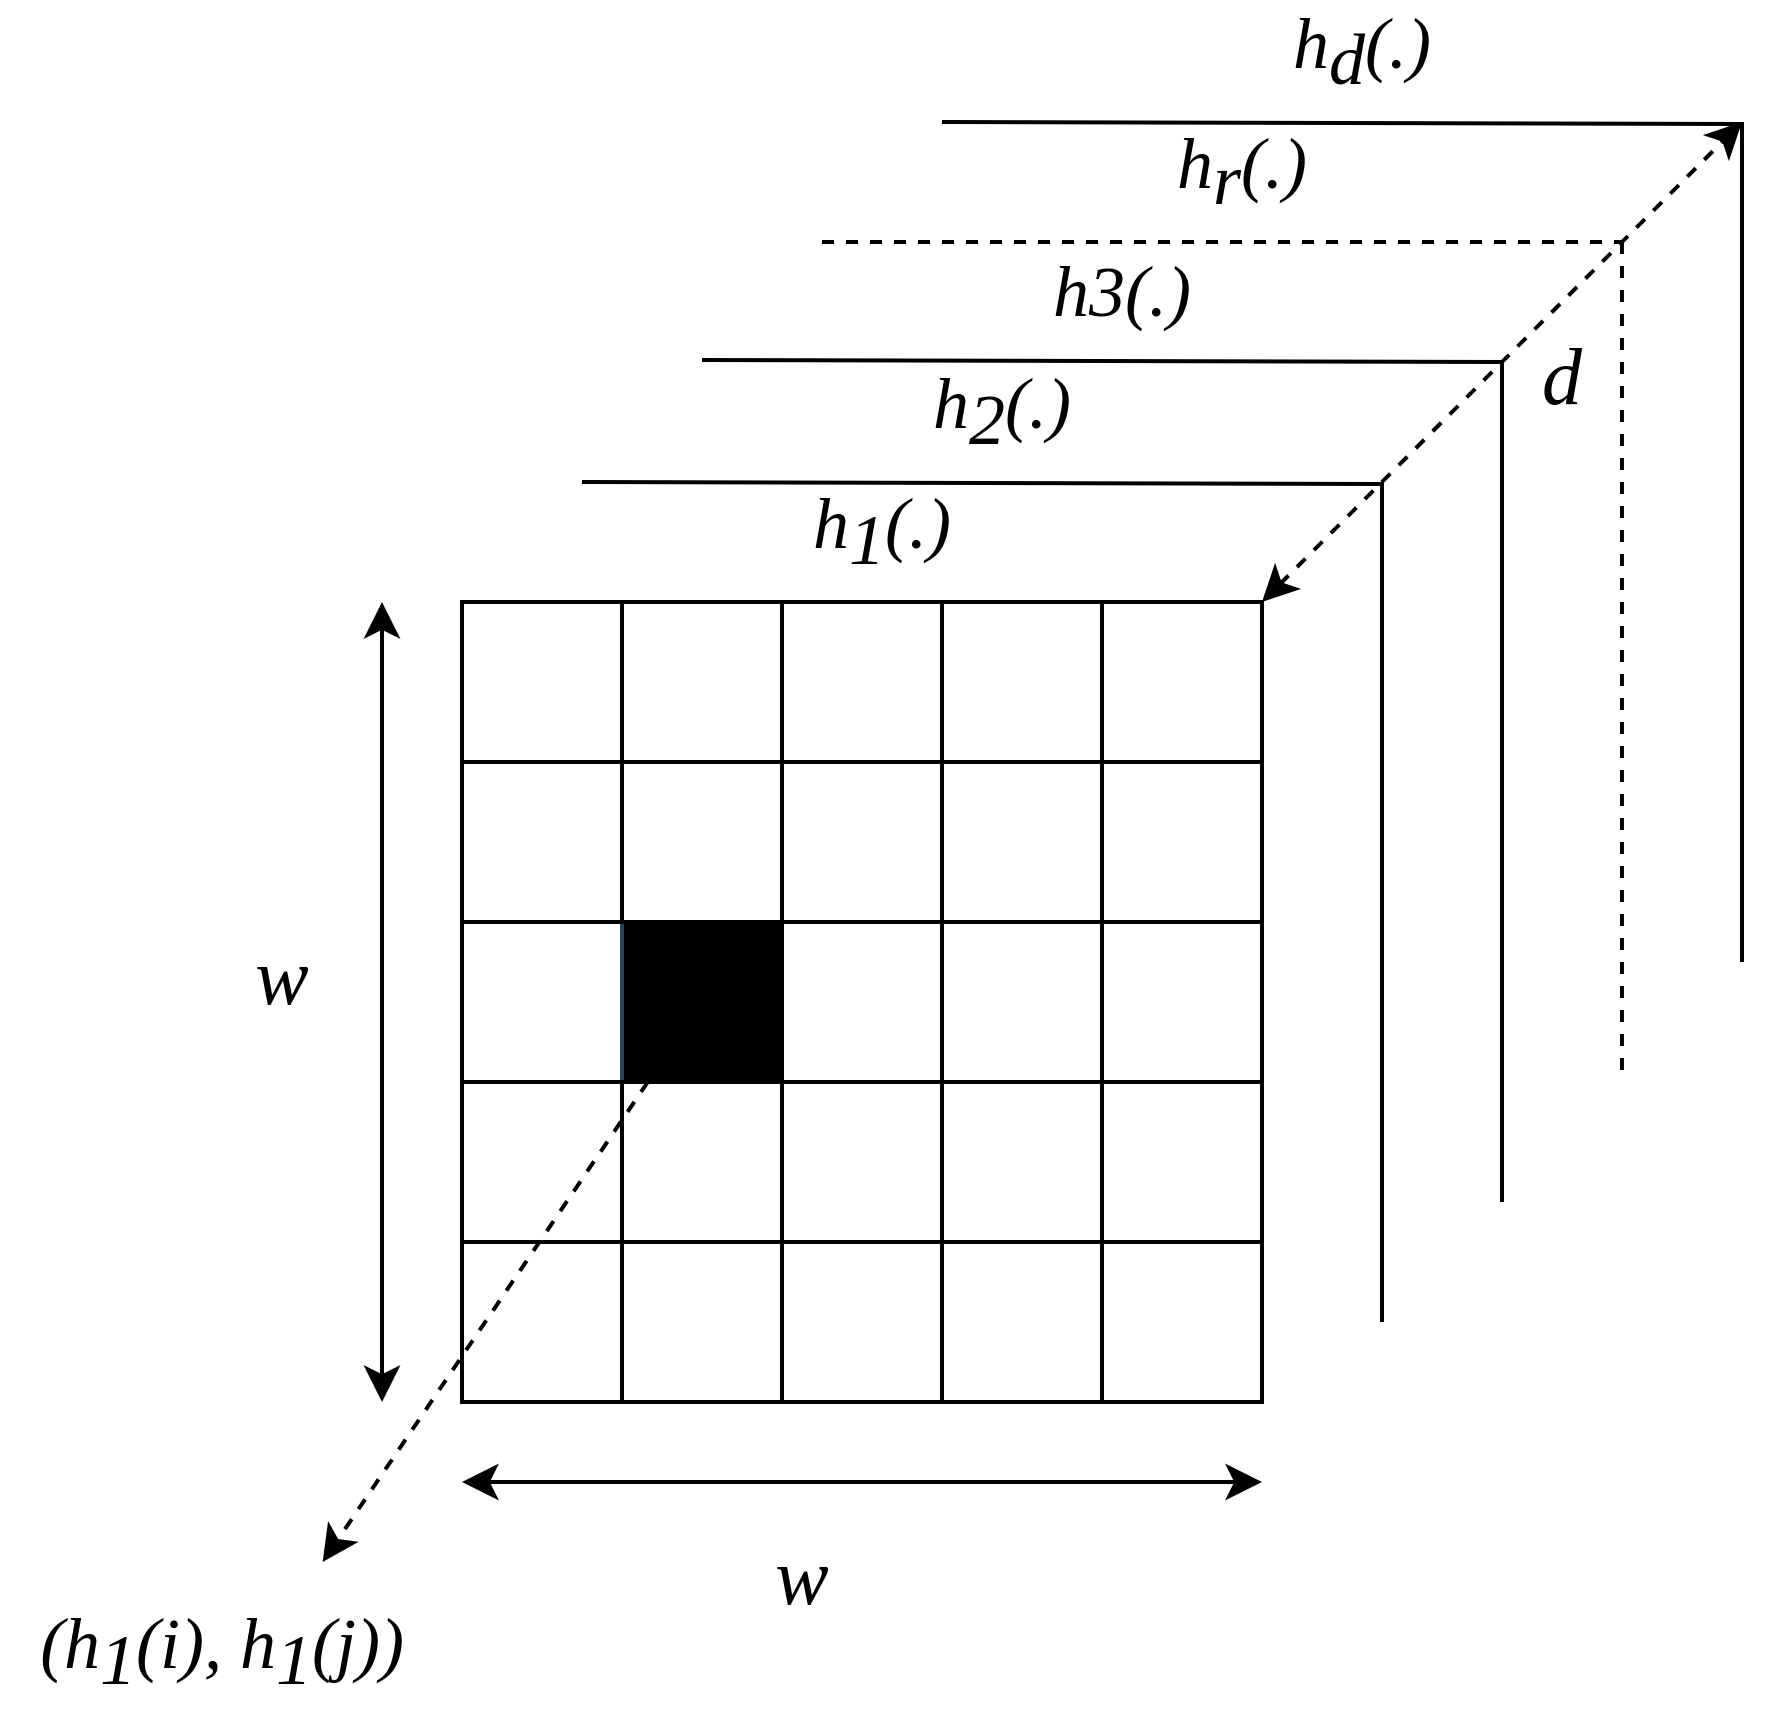
\includegraphics[width=0.7\textwidth]{tcm}
    \caption{TCM sketch}
    \label{fig:tcm}
\end{figure}

\subsubsection{GMatrix\cite{khan_query-friendly_2016}}

\paragraph{}
gMatrix is very similar to TCM and it was proposed in the same year as the TCM. However, gMatrix paper consider about,

\begin{itemize}
    \item reverse hashing queries through pairwise independent hash functions;
    \item alternative options to extend sketch and space-saving synopses for achieving similar functionalities as gMatrix;
\end{itemize}

which the TCM paper does not address.

\subsubsection{GSS\cite{gou_fast_2018}}

\paragraph{}
GSS is the latest graph summarization technique that has been introduced up to date which was published in 2018. Even when using 1/256 memory size of the state of the art graph summarization algorithm, GSS still significantly outperformed it for most queries. The GSS paper points out that even if TCM and gMatrix support all queries in the streaming graphs in contrast to CM sketches\cite{cormode_improved_2003} and gSketch which only supports queries for edges and do not get involved with the topology of the underlying graph, they suffer from poor accuracy. GSS improves upon TCM and gMatrix to increase the accuracy with less memory usage.

\paragraph{}
GSS defines three graph primitives as,

\begin{itemize}
    \item Edge query
    \item 1-hop Successor query
    \item 1-hop Precursor query
\end{itemize}

\paragraph{}
By supporting all these 3 types of queries it is possible to reconstruct the entire graph. Therefore it is also possible to run any kind of query against a sketch which supports all 3 of the above primitives.

\paragraph{}
The intuition behind the basic version of the GSS can be illustrated as below.

\begin{figure}[H]
    \centering 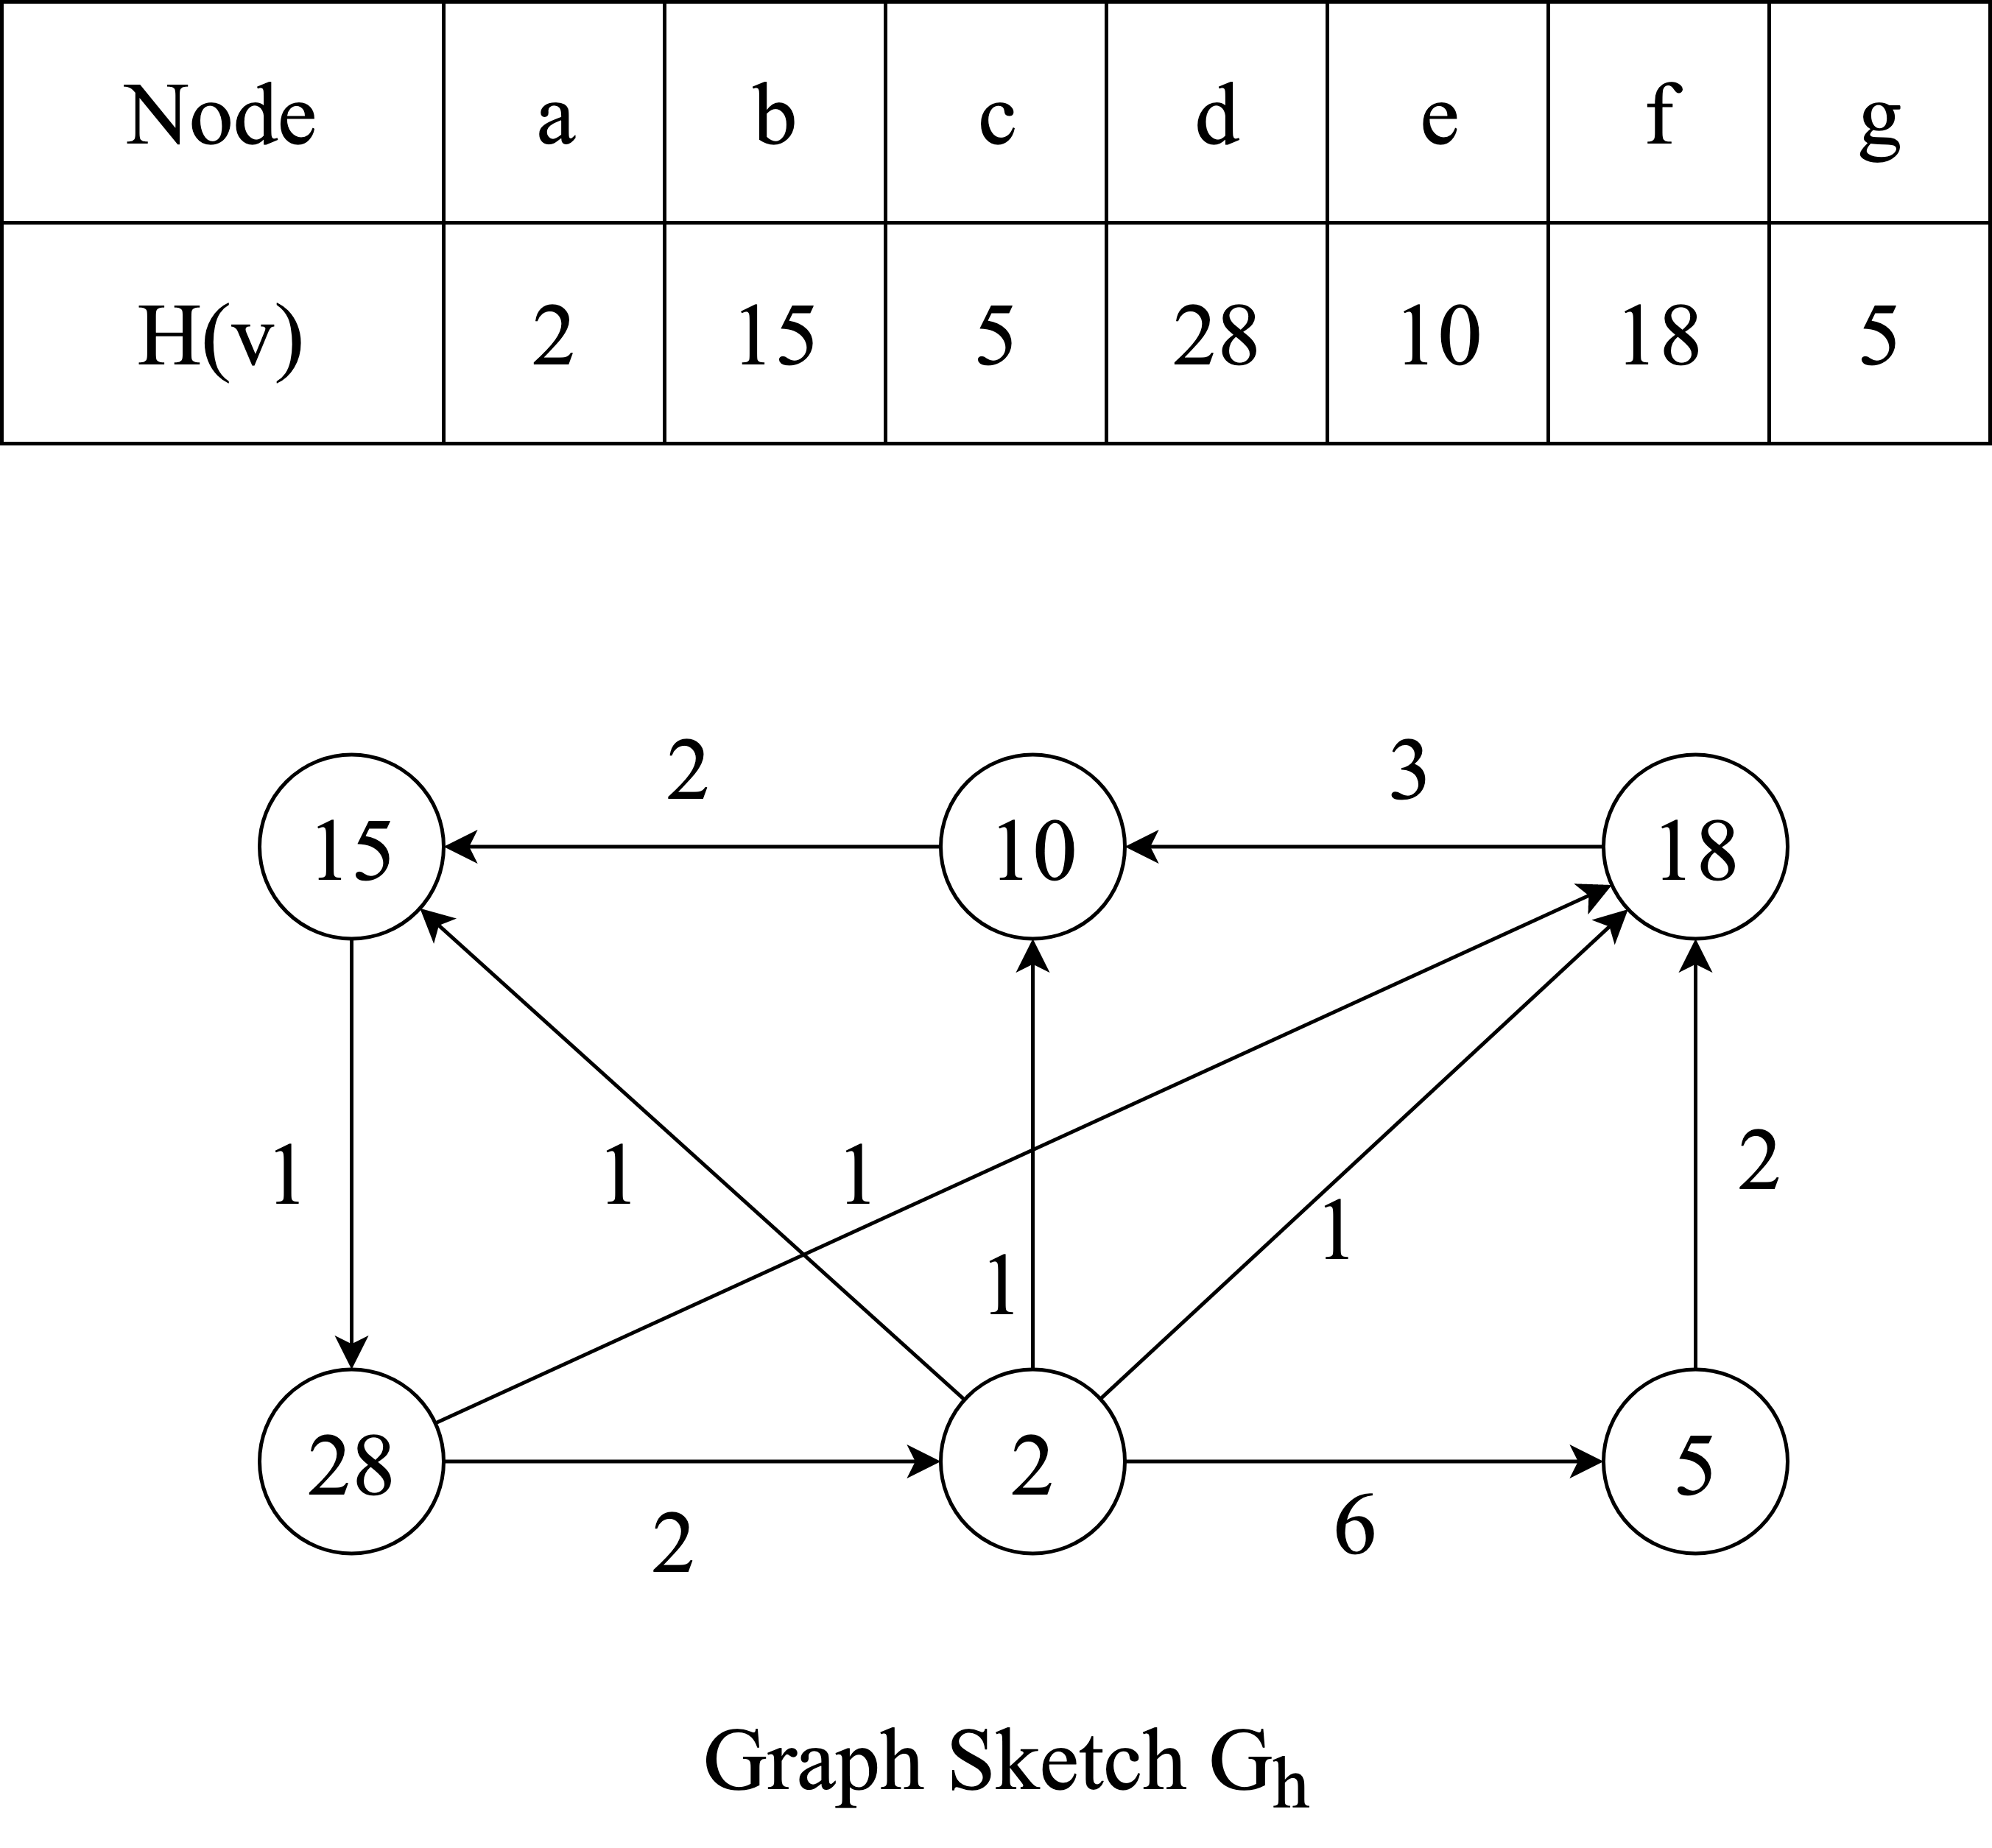
\includegraphics[width=0.6\textwidth]{gss1}
    \caption{A sample map function\cite{gou_fast_2018}}
    \label{fig:gss1}
\end{figure}

\paragraph{}
\(H(.)\) is a hash function which is used on the vertices of the original graph stream to create the graph sketch \(G\textsubscript{h}\) as indicated in Figure \ref{fig:gss1}.

\paragraph{}
A GSS sketch consists of two parts,

\begin{enumerate}
    \item Adjacency matrix
    \item List buffer B for leftover edges
\end{enumerate}

\paragraph{}
For each node in the sketch graph \(G\textsubscript{h}\), an address \(h(v)\) and a fingerprint \(f(v)\) is defined. Each edge \(H(s)\), \(H(d)\) is mapped into a bucket in the row \(h(s)\), column \(h(d)\) of the matrix. \([\langle f(s), f(d)\rangle, w]\) is recorded in the corresponding bucket of the matrix, where \(w\) is the edge weight and \(f(s)\), \(f(d)\) are the fingerprints for the source and destination. This can be seen in the sample of GSS sketch shown in Figure \ref{fig:gss2}.

\begin{figure}[H]
    \centering
    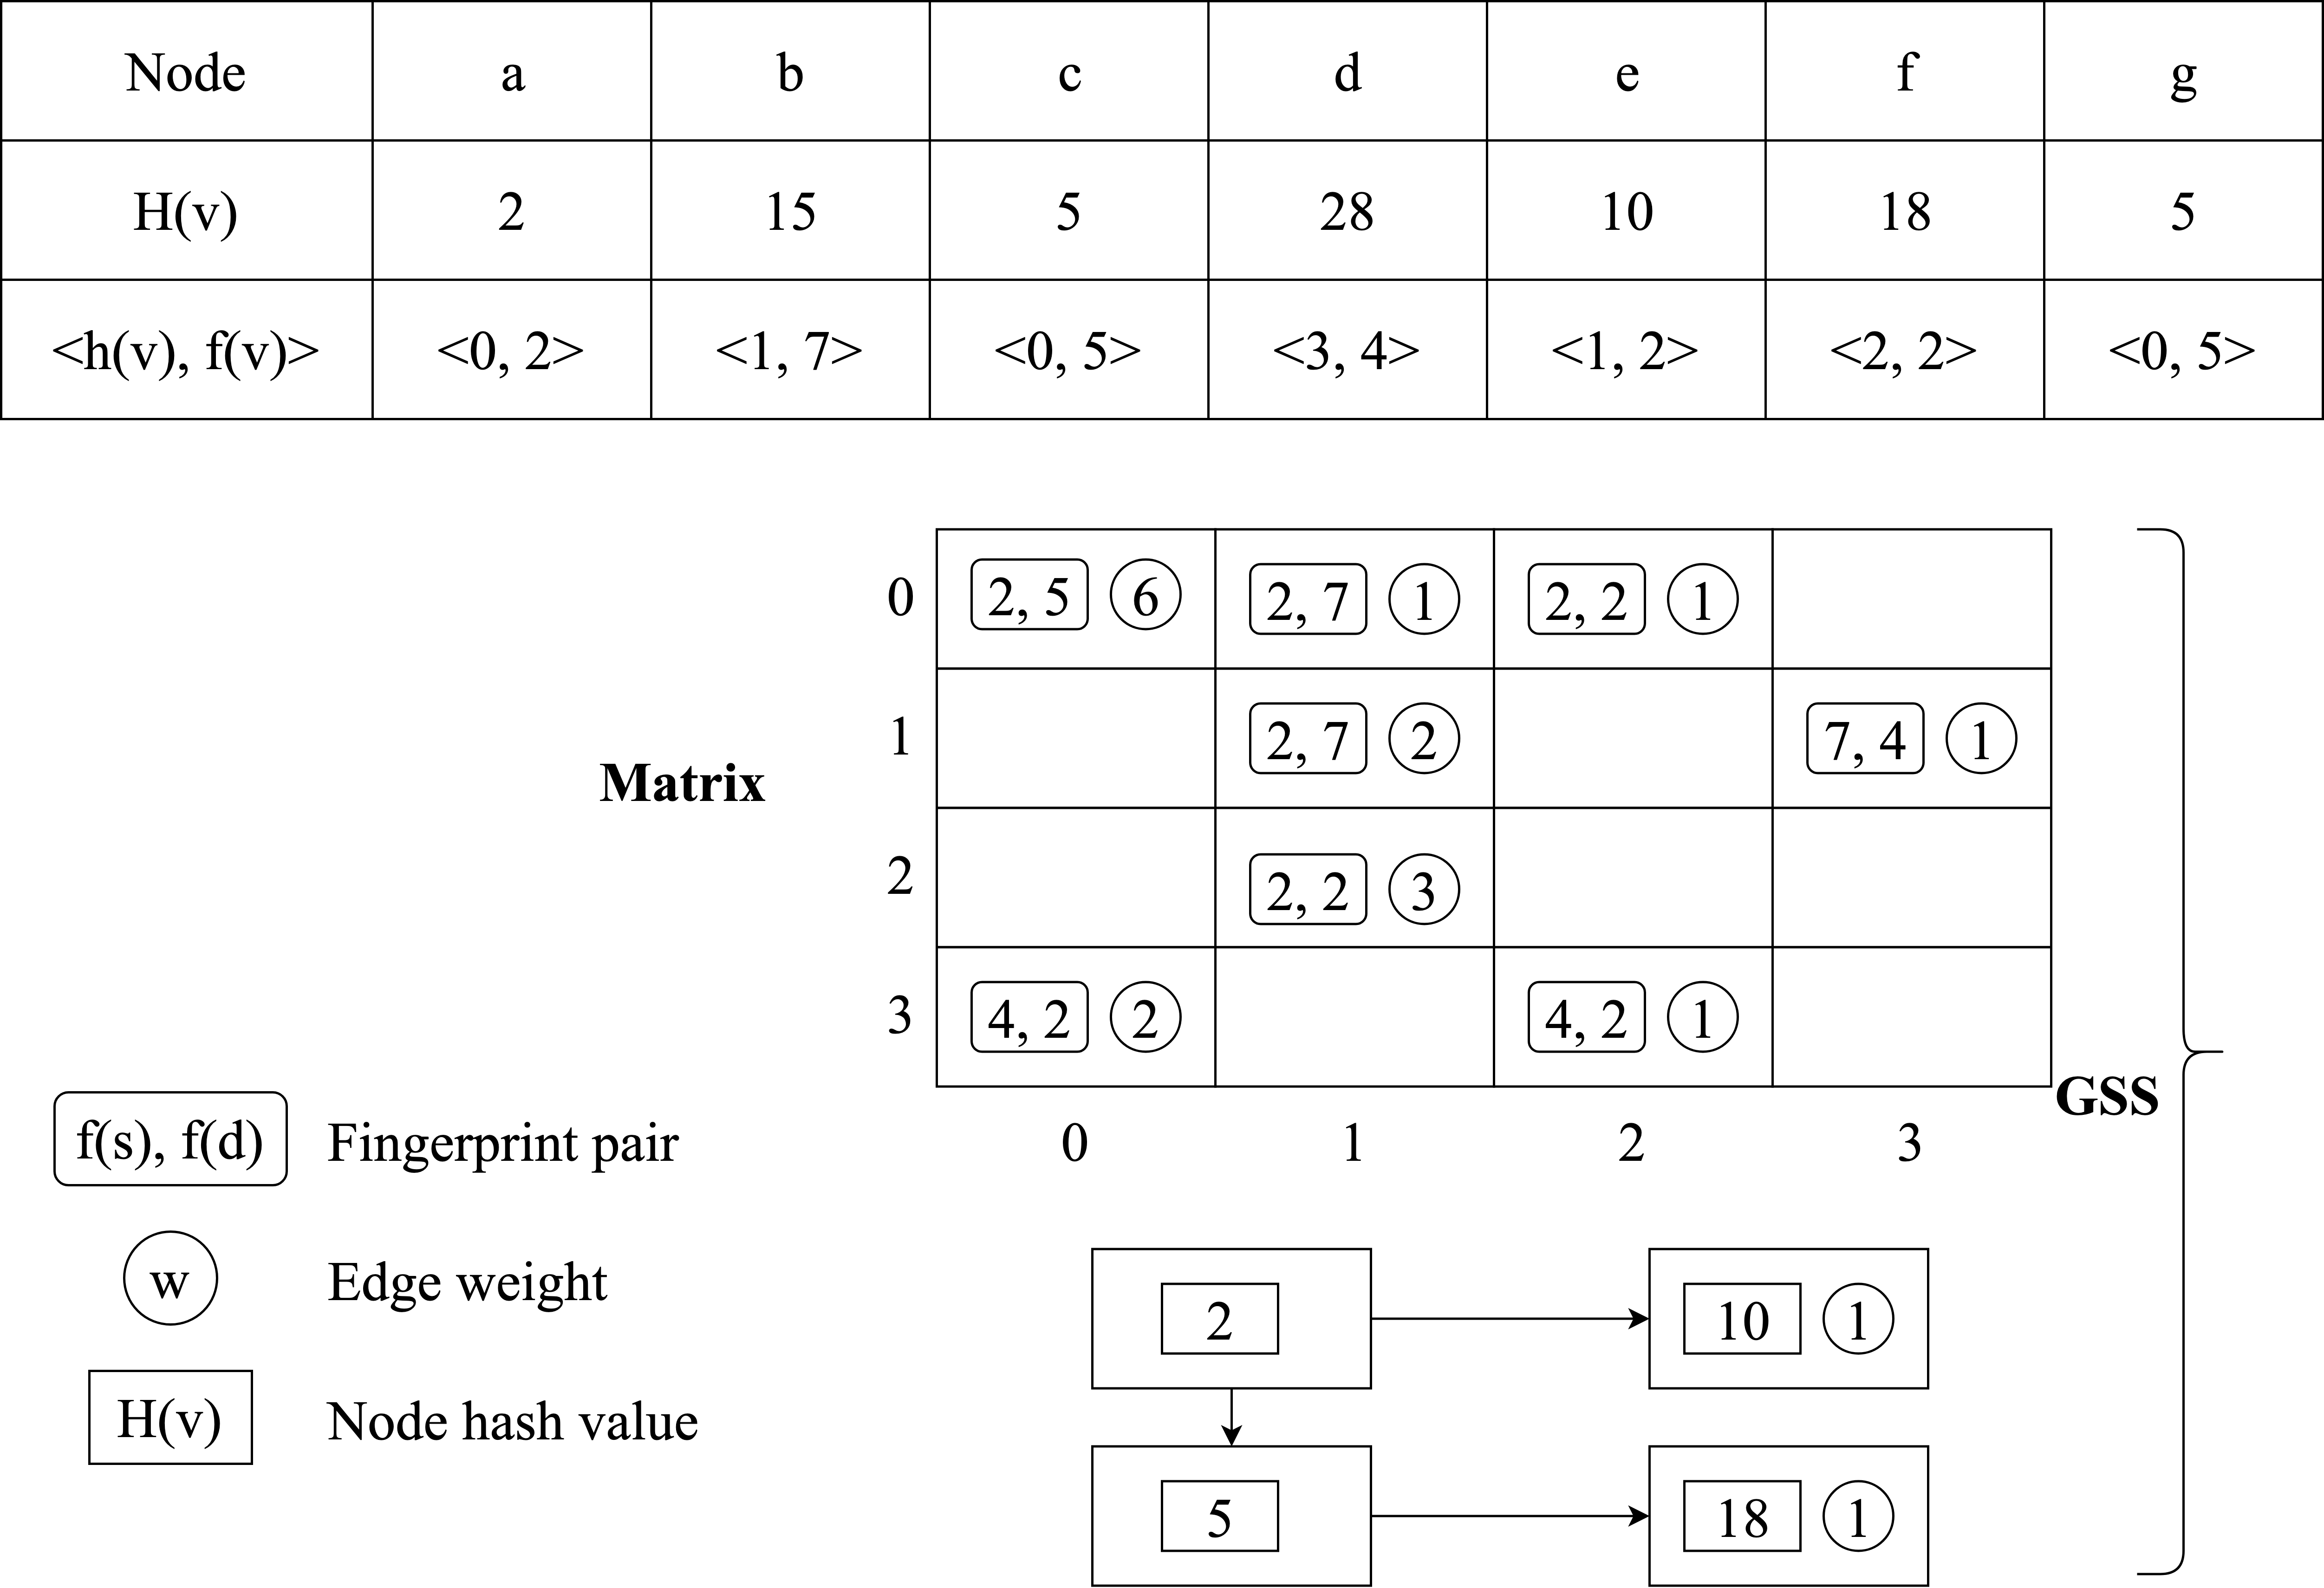
\includegraphics[width=\textwidth]{gss2}
    \caption{A sample version of the basic data structure\cite{gou_fast_2018}}
    \label{fig:gss2}
\end{figure}